% !TeX program = pdflatex
\documentclass[border=6pt]{standalone}
\usepackage{tikz}
\usetikzlibrary{arrows.meta, positioning, calc}

\definecolor{MediumRed}{rgb}{0.925, 0.345, 0.345}
\definecolor{MediumGreen}{rgb}{0.37, 0.7, 0.66}
\definecolor{MediumBlue}{rgb}{0.015, 0.315, 0.45}
\definecolor{DarkBlue}{rgb}{0.05, 0.15, 0.35}

\begin{document}
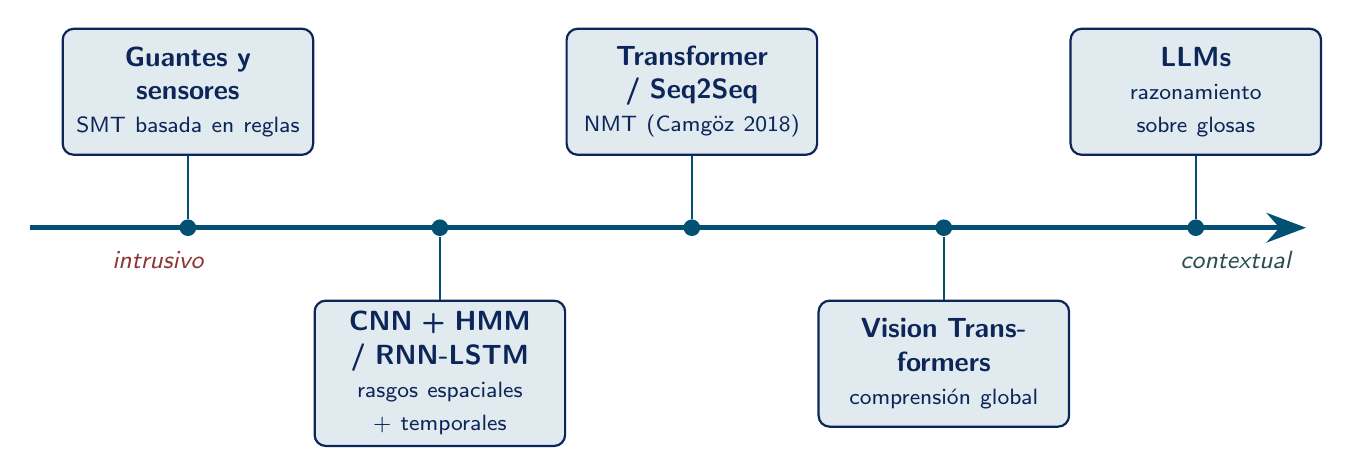
\begin{tikzpicture}[
    font=\sffamily,
    milestone/.style={draw=DarkBlue, thick, rounded corners=4pt,
        fill=MediumBlue!12, text=DarkBlue, align=center,
        text width=2.9cm, minimum height=1.6cm, inner sep=4pt},
    dot/.style={circle, fill=MediumBlue, minimum size=6pt, inner sep=0pt},
]

% eje temporal
\draw[-{Stealth[length=5mm]}, line width=2pt, MediumBlue] (-0.6,0) -- (15.6,0);

\foreach \x/\lbl/\dir [count=\i] in {%
    1.4/{\textbf{Guantes y sensores}\\\footnotesize SMT basada en reglas}/1,
    4.6/{\textbf{CNN + HMM / RNN-LSTM}\\\footnotesize rasgos espaciales + temporales}/-1,
    7.8/{\textbf{Transformer / Seq2Seq}\\\footnotesize NMT (Camg\"oz 2018)}/1,
    11.0/{\textbf{Vision Transformers}\\\footnotesize comprensión global}/-1,
    14.2/{\textbf{LLMs}\\\footnotesize razonamiento sobre glosas}/1%
}{
    \node[dot] (d\i) at (\x,0) {};
    \ifnum\dir=1
        \node[milestone, above=0.8cm of d\i] (m\i) {\lbl};
    \else
        \node[milestone, below=0.8cm of d\i] (m\i) {\lbl};
    \fi
    \draw[MediumBlue, thick] (d\i) -- (m\i);
}

% extremos: intrusivo -> contextual
\node[font=\sffamily\small\itshape, text=MediumRed!60!black, below left=0.1cm and -0.4cm of d1] {intrusivo};
\node[font=\sffamily\small\itshape, text=MediumGreen!45!black, below right=0.1cm and -0.4cm of d5] {contextual};

\end{tikzpicture}
\end{document}
